\documentclass{article}
\usepackage[margin=1in]{geometry}
\usepackage{problemset}
\showsolntrue

% Custom commands
\newcommand{\R}{\mathbb{R}}
\newcommand{\X}{\mathcal{X}}
\newcommand{\Y}{\mathcal{Y}}

\begin{document}

\pstitle{%
    CSE 151A%
}{
    Homework 8%
}[due Thursday, May 29 at 11:59PM]

\textbf{Instructions:}
\begin{itemize}
    \item You may discuss problems with your study group, but ultimately all your work (mathematical problems, code, experimental details) must be individual.
    \item Your solutions must be \texttt{typed up} and uploaded to Gradescope by 11.59PM on Thursday May 29. No late homeworks will be accepted under any circumstances, so you are encouraged to upload early.
    \item A subset of the problems will be graded.
\end{itemize}

\begin{probset}
\begin{prob}
    A linear predictor is used to solve a classification problem with three classes. The data is two-dimensional and the linear functions for each class are:

    \begin{enumerate}
        \item Class 1: $w_1 = \begin{bmatrix} 1 \\ 1 \end{bmatrix}$, $b_1 = 0$
        \item Class 2: $w_2 = \begin{bmatrix} 1 \\ 0 \end{bmatrix}$, $b_2 = 1$
        \item Class 3: $w_3 = \begin{bmatrix} 0 \\ 1 \end{bmatrix}$, $b_3 = -1$
    \end{enumerate}

    Draw the resulting decision boundary and clearly mark the region corresponding to each class.

    \begin{soln}
        Red is class 1, green is class 2, and purple is class 3.
        \begin{center}
            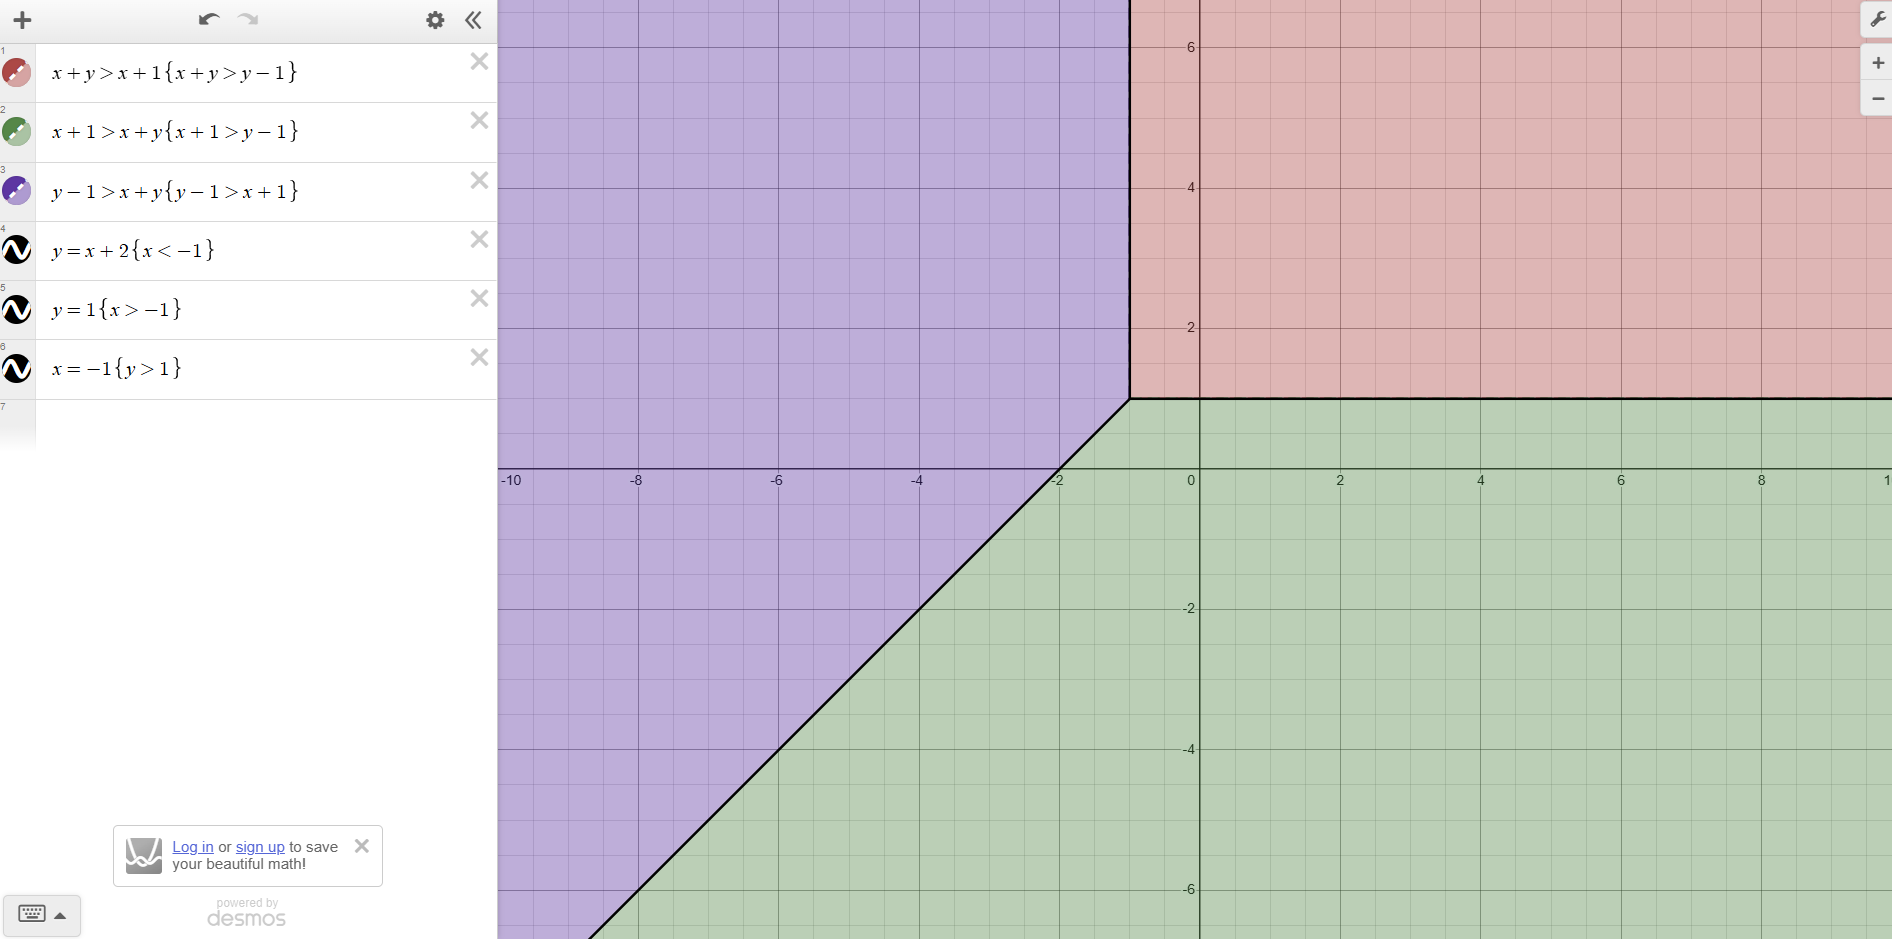
\includegraphics[width=0.8\textwidth]{Images/1.png}
        \end{center}
    \end{soln}
\end{prob}

\newpage

\begin{prob}
    Decision trees have great expressive power: they can represent any decision boundary, by carving up the space to a fine enough granularity. Which of the other methods we've studied are similarly expressive? For each, give a brief explanation.

    \begin{subprobset}
    \begin{subprob}
        Linear classifiers

        \begin{soln}
            Linear classifiers can only represent linear decision boundaries so they are not as expressive as decision trees.
        \end{soln}
    \end{subprob}

    \begin{subprob}
        Nearest neighbors classifiers

        \begin{soln}
            Nearest neighbors classifiers are very expressive, in the limit of 1-nearest neighbor and with sufficient data, they can approximate any decision boundary like decision trees.
        \end{soln}
    \end{subprob}

    \begin{subprob}
        Classifiers based on Gaussian generative models

        \begin{soln}
            While Gaussian generative models can represent non-linear decision boundaries, they are not as expressive as decision trees because they can only represent quadratic boundaries.
        \end{soln}
    \end{subprob}
    \end{subprobset}
\end{prob}

\begin{prob}
    In order to grow a decision tree, we need a measure of how pure or impure (in terms of labels) a node is. A popular measure of this is the Gini impurity index. If there are two labels, and a node has p fraction of one label and $1 - p$ fraction of the other, the Gini impurity index is $2p(1 - p)$. Notice that this is maximized when $p = 1/2$.

    What is the Gini impurity index for a node in which 20\% of the points have one label while 80\% have the other label?

    \begin{soln}
        $2 \cdot 0.2 \cdot (1 - 0.2) = 0.32$
    \end{soln}
\end{prob}

\newpage

\begin{prob}[\textit{Working with weighted data}]
    Boosting requires the weak learning algorithm to work with training data in which each point $(x^{(i)}, y^{(i)})$ has a positive weight $\lambda_i > 0$. Intuitively, a weight of two would be equivalent to having two copies of that data point. How would you incorporate weights into the following learning algorithms without explicitly making copies of data points? Give a brief explanation in each case.

    \begin{subprobset}
    \begin{subprob}
        Decision trees.

        \textit{Hint:} Previously, we measured the uncertainty at any node by looking at the fraction of points with each label (call these $p_1, \ldots, p_k$ if there are $k$ labels). Now we need to compute these fractions differently, taking weights $\lambda_i$ into account.

        \begin{soln}
            We can use the weights to compute the uncertainty at any node by looking at the weighted fraction of points with each label. That is, use the following to compute the fraction of points with label $j$:
            \[
                p_j = \frac{\sum_{i: y^{(i)} = j} \lambda_i}{\sum_{i} \lambda_i}
            \]
        \end{soln}
    \end{subprob}

    \begin{subprob}
        Gaussian generative models.

        \textit{Hint:} For each class $j$, we need the weight of that class ($\pi_j$), the mean ($\mu_j$), and the covariance matrix ($\Sigma_j$). Now we need to compute them differently, taking weights $\lambda_i$ into account.

        \begin{soln}
            We can use the weights to compute the weight of each class by:
            \[
                \pi_j = \frac{\sum_{i: y^{(i)} = j} \lambda_i}{\sum_{i} \lambda_i}
            \]
            and the mean and covariance matrix by:
            \[
                \mu_j = \frac{\sum_{i: y^{(i)} = j} \lambda_i x^{(i)}}{\sum_{i: y^{(i)} = j} \lambda_i}
            \]
            and
            \[
                \Sigma_j = \frac{\sum_{i: y^{(i)} = j} \lambda_i (x^{(i)} - \mu_j)(x^{(i)} - \mu_j)^T}{\sum_{i: y^{(i)} = j} \lambda_i}
            \]
        \end{soln}
    \end{subprob}

    \begin{subprob}
        Support vector machines.

        \textit{Hint:} Can you incorporate the weights $\lambda_i$ into the objective function for soft-margin SVM?

        \begin{soln}
            We can incorporate the weights into the objective function for soft-margin SVM by multiplying the loss term by the weight of the point:
            \[
                \min_{w, b, \xi} \frac{1}{2}\|w\|^2 + C \sum_{i} \lambda_i \xi_i
            \]
            subject to the constraints:
            \[
                y^{(i)}(w^T x^{(i)} + b) \geq 1 - \xi_i, \quad \xi_i \geq 0.
            \]
        \end{soln}
    \end{subprob}
    \end{subprobset}
\end{prob}

\newpage

\begin{prob}[\textit{Convergence behavior of boosting}]
    Suppose we run boosting using weak classifiers from some class $H$ (such as decision stumps), and suppose that on each round, the weak learner always returns a weak classifier whose error rate on the weighted data (for that round) is at most $1/2 - \epsilon$, for some $\epsilon > 0$. Which of the following is true? Give a brief explanation in each case.

    \begin{subprobset}
    \begin{subprob}
        Boosting converges to a final classifier with zero test error.

        \begin{soln}
             This is not necessarily true. Boosting aims to reduce training error, but generalization depends on factors like noise in data, model complexity, and overfitting. So, it does not guarantee zero test error.
        \end{soln}
    \end{subprob}

    \begin{subprob}
        Boosting converges to a final classifier with zero training error.

        \begin{soln}
            This is true. If each weak learner performs better than random guessing by at least $\epsilon$ (i.e., error $\leq \frac{1}{2} - \epsilon$), then boosting is guaranteed to reduce the training error exponentially fast and will eventually reach zero training error, assuming the data is separable.
        \end{soln}
    \end{subprob}

    \begin{subprob}
        Boosting's final classifier belongs to class $H$.

        \begin{soln}
            This is not necessarily true. The final classifier is a weighted combination of many classifiers from $H$, not a single member of $H$. So the final hypothesis may lie outside $H$.
        \end{soln}
    \end{subprob}
    \end{subprobset}
\end{prob}

\begin{progprob}[\textit{Multiclass Perceptron}]
    Implement the multiclass Perceptron algorithm from class. Then, load in the data set \texttt{data0.txt}. This has 2-d data in four classes (coded as 0,1,2,3). Each row consists of three numbers: the two coordinates of the data points and the label.

    Run the multiclass Perceptron algorithm to learn a classifier. Turn in a plot that shows all the data points (with different colors and shapes for different labels) as well as the decision regions.

    \begin{soln}
        \begin{center}
            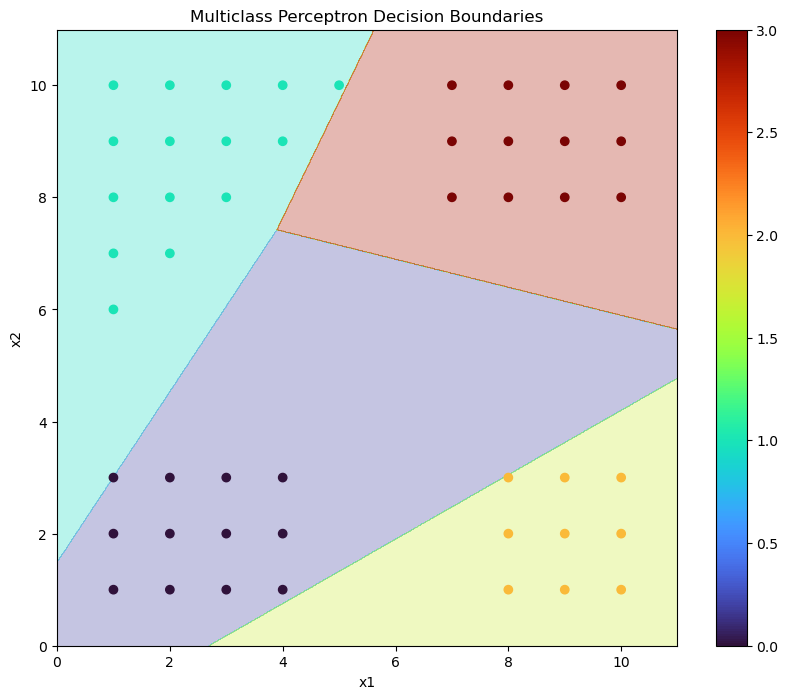
\includegraphics[width=0.55\textwidth]{Images/6.png}
        \end{center}
    \end{soln}
\end{progprob}

\newpage

\begin{progprob}[\textit{Multiclass SVM}]
    In this problem, we'll use support vector machines on the same data set, \texttt{data0.txt}.

    \begin{itemize}
        \item Learn a linear SVM classifier using \texttt{sklearn.svm.LinearSVC}. You will need to set \texttt{loss='hinge'} and \texttt{multi\_class='crammer\_singer'}. Try the following values of $C$: 0.01, 0.1, 1.0, 10.0.
    \end{itemize}

    \begin{subprobset}
    \begin{subprob}
        For each value of $C$, plot the decision boundary (no need to show the margins).

        \begin{soln}
            \begin{center}
                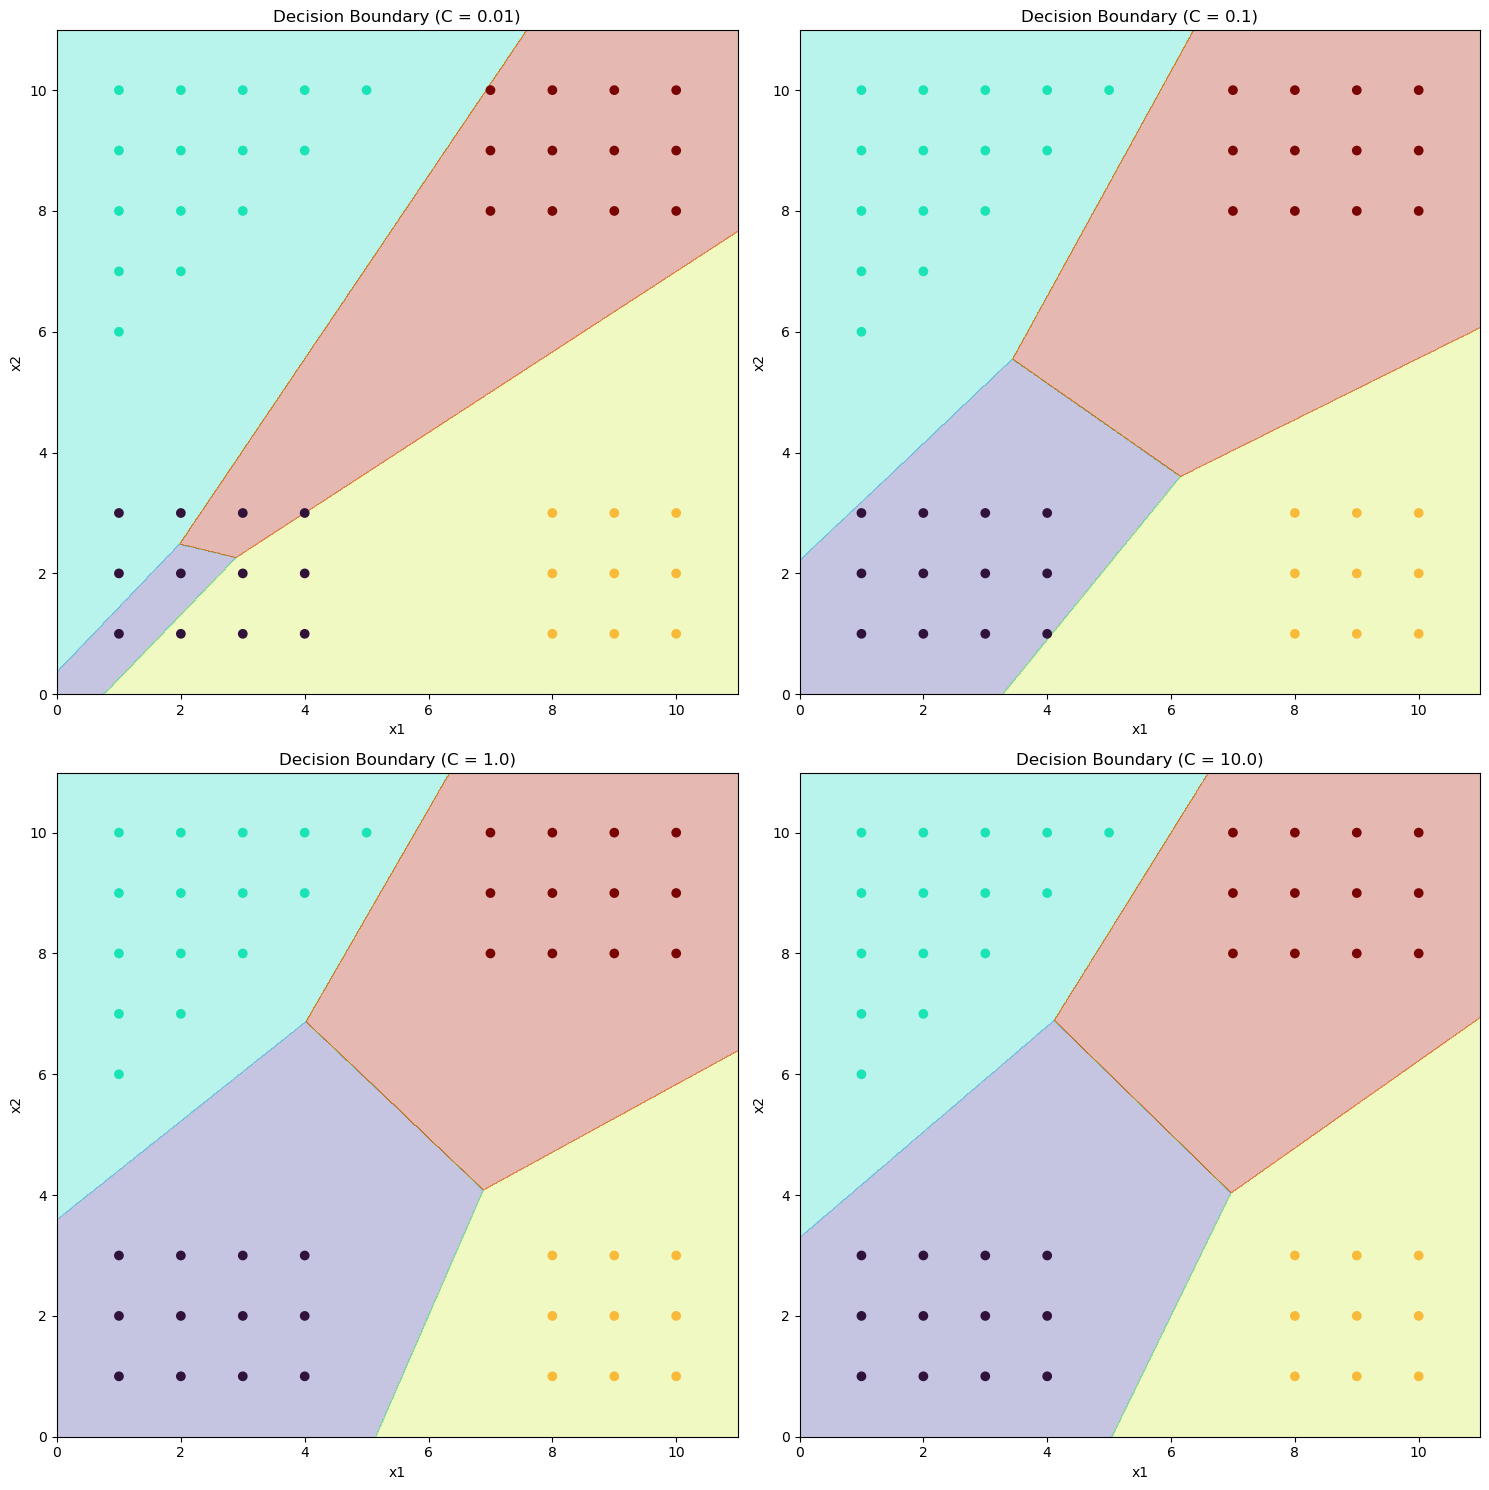
\includegraphics[width=0.55\textwidth]{Images/7.png}
            \end{center}
        \end{soln}
    \end{subprob}

    \begin{subprob}
        What do you notice as $C$ increases? Briefly comment.

        \begin{soln}
            Although the accuracy of the classifier hits 100\% for $C \geq 0.1$, the larger $C$ values (1 and 10) show more reasonable decision boundaries in terms of generalization. This is better than the Perceptron algorithm, which stops as soon as it reaches 100\% training accuracy which may not generalize well.
        \end{soln}
    \end{subprob}
    \end{subprobset}
\end{progprob}

\newpage

\begin{progprob}[\textit{A toy 2-d data set for decision trees and boosting}]
    Obtain the data set \texttt{mini-data.txt} from the course webpage. Each line has a two-d data point followed by a label (0 or 1).

    \begin{subprobset}
    \begin{subprob}
        Plot this data to see what it looks like. Show this plot in your writeup.

        \begin{soln}
            \begin{center}
                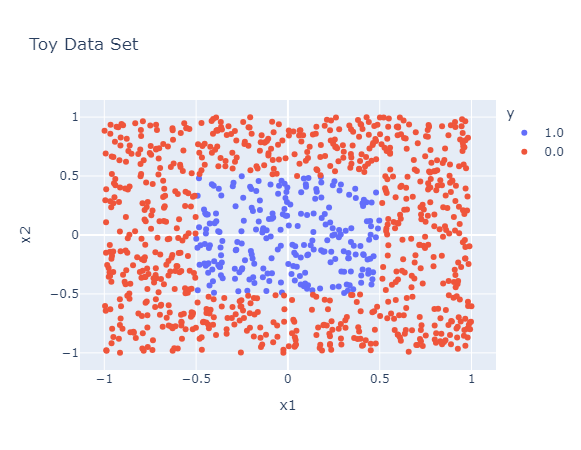
\includegraphics[width=0.6\textwidth]{Images/8a.png}
            \end{center}
        \end{soln}
    \end{subprob}

    \begin{subprob}
        Use \texttt{sklearn.tree.DecisionTreeClassifier} to fit a decision tree to the data. What stopping criterion did you use?

        \begin{soln}
            I used a max depth of 4 because drawing 4 lines would isolate the rectangle in which all the points classified as 1 reside.
        \end{soln}
    \end{subprob}

    \begin{subprob}
        Display the tree using \texttt{sklearn.tree.plot\_tree}.

        \begin{soln}
            \begin{center}
                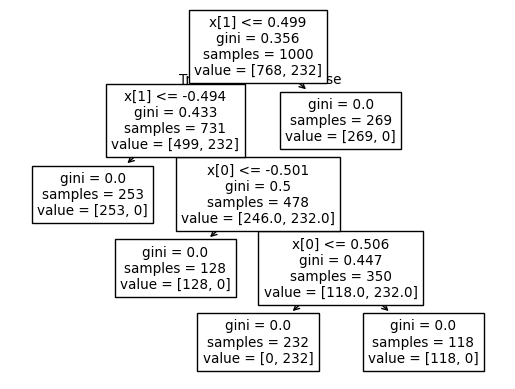
\includegraphics[width=0.6\textwidth]{Images/8c.png}
            \end{center}
        \end{soln}
    \end{subprob}

    \newpage

    \begin{subprob}
        Fit boosted decision stumps to this data using \texttt{sklearn.ensemble.AdaBoostClassifier}. Use a relatively small number of stumps, and display each of them.

        \begin{soln}
            \begin{center}
                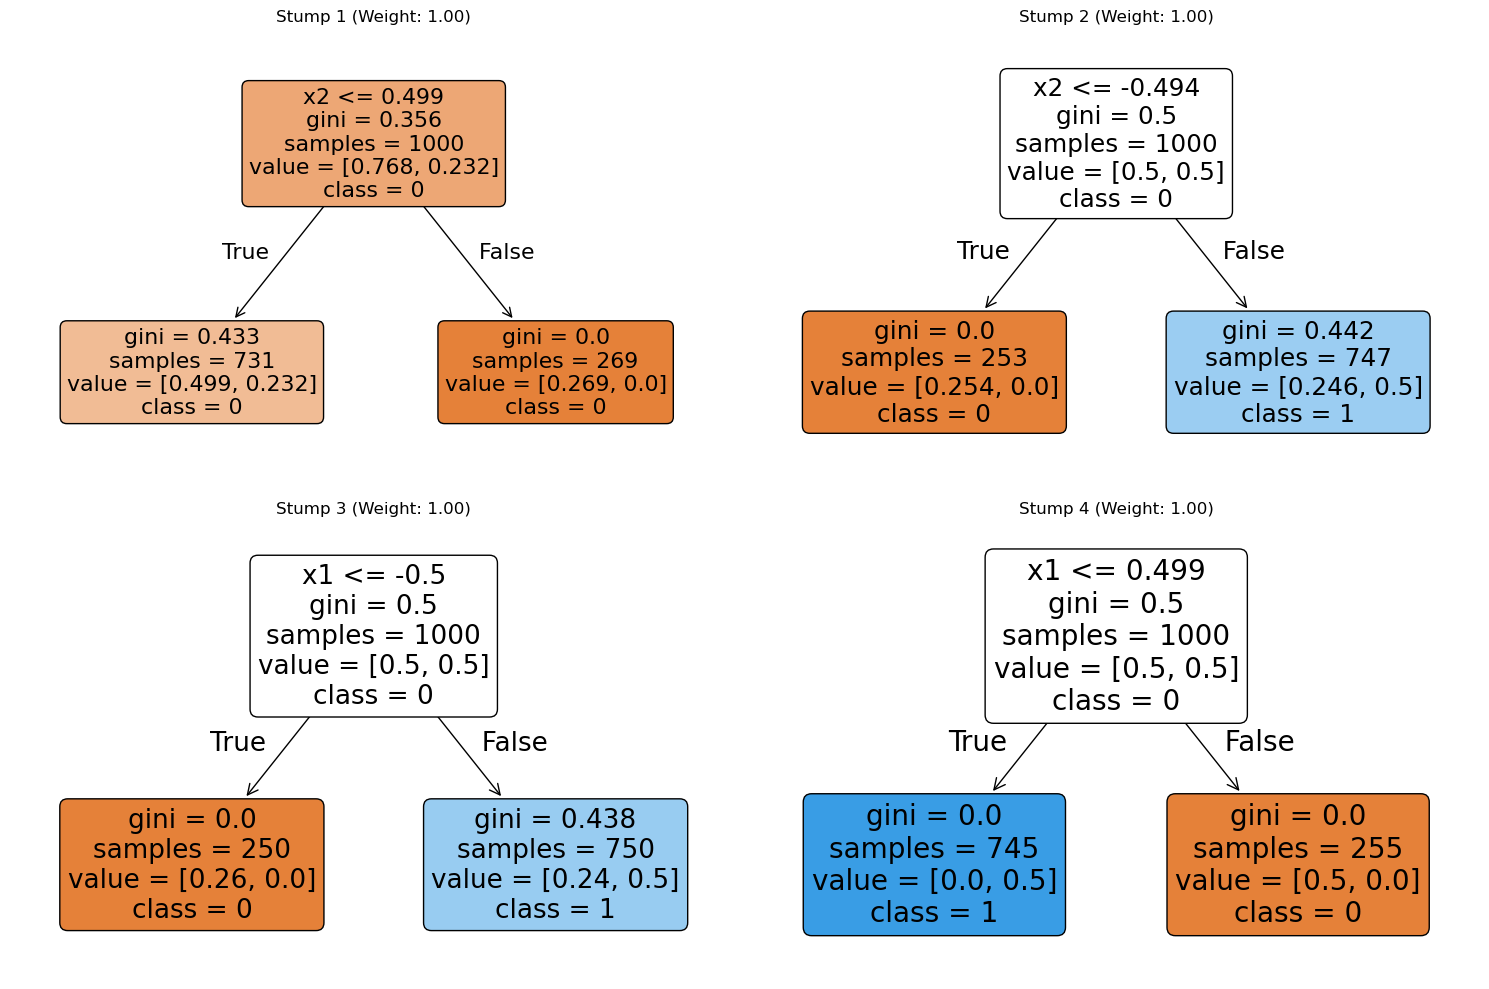
\includegraphics[width=0.8\textwidth]{Images/8d.png}
            \end{center}
        \end{soln}
    \end{subprob}

    \begin{subprob}
        Give a table showing how accuracy on the training data improves as each successive stump is added.

        \begin{soln}
            \begin{center}
                \begin{tabular}{cc}
                    \toprule
                    Stumps & Accuracy \\
                    \midrule
                    1 & 0.768 \\
                    2 & 0.768 \\
                    3 & 0.882 \\
                    4 & 1.000 \\
                    \bottomrule
                \end{tabular}
            \end{center}
        \end{soln}
    \end{subprob}
    \end{subprobset}
\end{progprob}
\end{probset}
\end{document}